\chapter{Power, Supervision, and Noise Architecture}
\label{chap:power}
% Traceability: ADR-001 ADR-003 ADR-005

Every standard backplane provides the same power interface. Each function board chooses which supplies to consume and which to generate locally. Shared rails and local conversion are combined according to the loads, noise limits, and thermal budget.

Power supervision follows the same division of responsibility. The backplane protects and supervises shared power. Each active board protects its own safety-related functions. The main board measures common rails to help the host diagnose a trip.

Figure~\ref{fig:power-tree} shows the complete power path and the main supervision paths.

\begin{figure}[htbp]
  \centering
  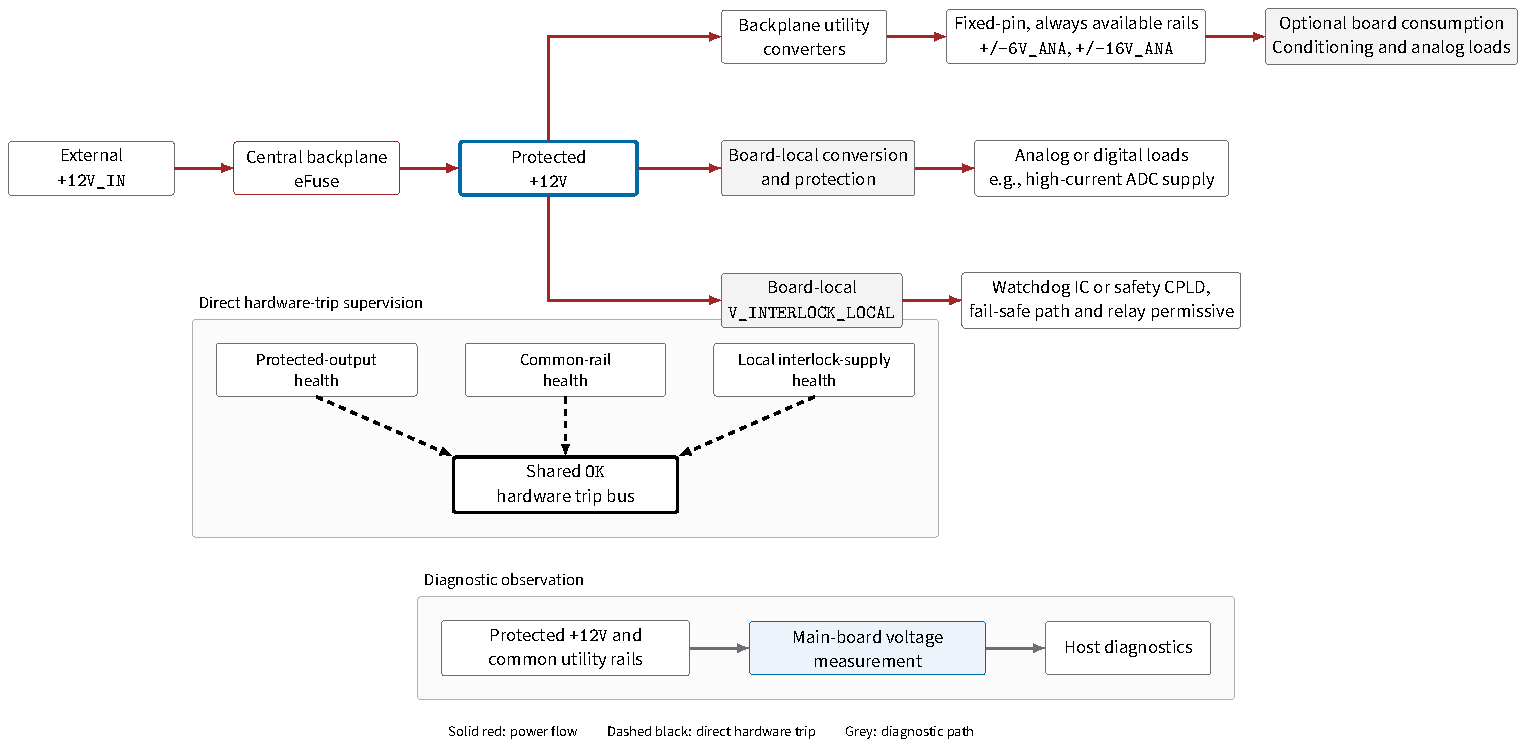
\includegraphics[width=\textwidth]{figures/generated/power_tree.tikz.pdf}
  \caption{Power and supervision overview. Red lines show power flow, dashed black lines show direct hardware contributions to the shared fault bus, and grey lines show diagnostic measurement.}
  \label{fig:power-tree}
\end{figure}

\section{What Power Is Available?}

\subsection{Protected bulk power}

The external system input is called \texttt{+12V\_IN}. It enters the backplane and passes through one central eFuse. The eFuse output is the protected rail called \texttt{+12V}.

The two names identify an important protection boundary:

\begin{center}
\texttt{+12V\_IN} $\longrightarrow$ central backplane eFuse $\longrightarrow$ protected \texttt{+12V}
\end{center}

The central eFuse acts as the system input circuit breaker. It protects against unsafe input voltage, reverse polarity, excessive total current, and system inrush. It also prevents the protected \texttt{+12V} rail from remaining outside the verified input range of downstream converters. If that range cannot be maintained, it disconnects all downstream power. The utility converters and every active board are behind this device.

The exact eFuse part, limits, delays, and restart behavior are backplane design choices. They are selected from the system power requirements and verified operating conditions.

\subsection{Common analog rails}

Shared analog utility supplies let boards reuse common conversion where it suits their loads. Ordinary digital supplies remain locally generated from protected \texttt{+12V}.

Every standard backplane provides the following utility rails on fixed connector assignments.

\providecommand{\GeneratedUtilityRailRows}{%
\texttt{+6V\_ANA} & Common positive low-voltage analog utility rail \\
\texttt{-6V\_ANA} & Common negative low-voltage analog utility rail \\
\texttt{+16V\_ANA} & Common positive analog utility rail \\
\texttt{-16V\_ANA} & Common negative analog utility rail \\
}


\begin{table}[htbp]
\centering
\begin{tabularx}{\textwidth}{@{}>{\bfseries}p{0.26\textwidth}>{\raggedright\arraybackslash}X@{}}
\toprule
Rail & Intended use \\
\midrule
\GeneratedUtilityRailRows
\bottomrule
\end{tabularx}
\caption{Standard backplane utility rails, generated from ADR-005.}
\label{tab:utility-rails}
\end{table}

A board does not have to consume every utility rail. An analog board may use several of them, while a specialized board may use only protected \texttt{+12V}. The standard interface remains the same in both cases. A backplane that removes or repurposes a standard rail is a separate architecture variant and needs an explicit decision and ICD.

\section{How a Board Uses the Available Power}

Function boards may use any subset of these rails, leave unused rail contacts unconnected, or generate supplies locally from protected \texttt{+12V}, even when an equivalent nominal voltage is available on the backplane. Local conversion is a normal application-dependent choice, not an architecture variant. A high-current ADC supply may use local conversion while other analog loads use shared rails. Voltage, current, noise, transient response, efficiency, and thermal requirements guide this choice.

Ordinary digital supplies are different. Each board generates its processor, FPGA, memory, identification, monitoring, and management supplies locally from protected \texttt{+12V}. The standard backplane does not distribute a low-voltage digital utility rail because no common use case justifies its converter, connector allocation, supervision, and shared-noise path.

\subsection{Local conversion and protection}

Processors, FPGAs, and memory can draw substantial current at low voltage. Distributing that current directly at 3.3~V would require more connector contacts and heavier copper. It would also increase voltage drop and expose a common rail to fast digital load changes from every board.

The architecture therefore sends protected \texttt{+12V} to each active board. The board converts it locally to the voltages needed by its processor, FPGA, memory, and other high-current loads. Higher distribution voltage keeps the shared current lower for the same delivered power. Local conversion also keeps fast point-of-load behavior close to the circuits that create it.

The same \texttt{+12V} rail is the normal source for uncommon detector voltages. A specialized bias board may need voltages that are not useful to the rest of the controller. Those converters remain on that board instead of adding uncommon rails to every backplane slot.


Each board is responsible for the loads behind its connector. Its ICD declares steady current, peak demand, inrush or input capacitance, voltage tolerance, and sequencing needs for every rail it consumes.

Both main and function boards may use optional input eFuses on protected \texttt{+12V} or any consumed analog utility rail, using protection circuitry suitable for the rail's voltage and polarity. A fuse, load switch, protected converter, or another suitable method may also provide local protection. The choice depends on the board's energy, failure, and service risks. What matters is that a board fault must not damage the board, connector, or shared distribution.

Common analog rails usually feed filters and LDOs at the board boundary. These circuits provide regulation and noise control, but they are not automatically circuit breakers. The architecture does not require a separate eFuse on every analog-rail input.

The architecture also does not require independent supervision of every local converter. A local monitor is added when failure of that rail or output could leave a safety-related function in a hazardous condition that is not already covered by the board's fail-safe and watchdog paths.

\subsection{Conditioning shared rails}

Every shared power rail connects the noise behavior of the boards that use it. This includes protected \texttt{+12V} as well as the shared analog utility rails. Incoming noise can disturb local circuitry, while a board can return load transients and conducted emissions to the rail and disturb another board.

Digital loads and board-local converters must also control the disturbances they inject into protected \texttt{+12V}. Another board may use that same bulk rail to generate sensitive analog supplies. Local conversion does not remove the shared input-noise path.

Each function board therefore conditions every consumed shared rail at its power-entry boundary. As shown in Figure~\ref{fig:shared-rail-noise}, the conditioning has two jobs:

\begin{enumerate}
  \item reduce incoming rail disturbances enough for the local circuitry; and
  \item limit disturbances returned by the board to the common rail.
\end{enumerate}

\begin{figure}[htbp]
  \centering
  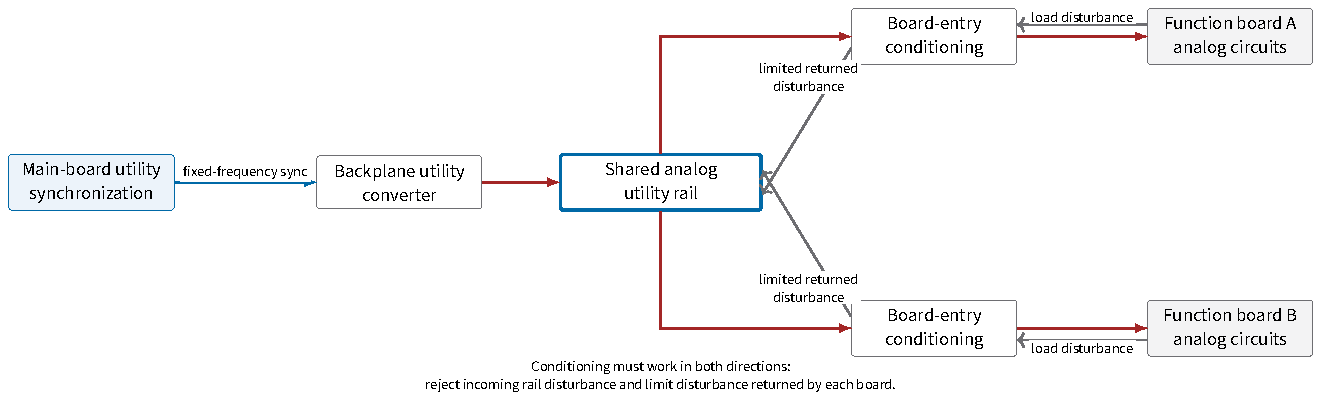
\includegraphics[width=\textwidth]{figures/generated/shared_rail_noise.tikz.pdf}
  \caption{Shared analog-rail example of bidirectional conditioning. The same incoming-noise and returned-disturbance requirements apply to protected \texttt{+12V}, including digital loads and local converters. Utility-converter synchronization makes the switching pattern predictable; conditioning does not imply zero noise.}
  \label{fig:shared-rail-noise}
\end{figure}

The board design may use an LDO, passive filter, ferrite and local storage, active filter, or another verified circuit. The architecture does not choose one topology or set component values. The backplane ICD defines the rail environment, and each function-board ICD declares the rejection it needs and the disturbance it is allowed to return.

\subsection{Returns, connectors, and budgets}

Power integrity also depends on return-current paths and connector allocation. The architecture does not require separate physical connectors for analog and digital signals. One connector can be used if its pinout and routing keep analog power, digital infrastructure, fast signals, and their returns in deliberate zones.

Analog-power and digital/infrastructure returns use dedicated contacts. Fast differential pairs have nearby returns. Analog utility contacts are separated from fast digital signals by return contacts or an equivalent grounded boundary. Chassis and shield connections remain distinct from circuit returns. The backplane design defines where analog and digital circuit returns are intentionally related.

Connector current capacity is not only a steady-state calculation. The design must also check contact resistance, voltage drop, temperature rise, inrush, peak demand, copper heating, and reliability. Parallel contacts are used where the verified current requires them.

The same rule applies to the complete controller. An empty physical slot does not prove that enough power, cooling, timing, or network capacity remains for another board. Integration checks the worst-case installed set of boards against the per-slot and total budgets.

\section{What Happens When Power Fails?}

\subsection{Complete input cutoff}
The eFuse is independent of the normal arm and fault state. A shared interlock trip makes detector-facing functions safe, but it does not normally turn off the complete controller. This allows boards to retain diagnostics and communicate with the host. The eFuse removes system power only when required by its own input-protection function.

If the eFuse disconnects the complete system, all active boards and powered outputs turn off. Normally-open detector relays also de-energize. The architecture does not require the shared fault bus or telemetry to remain active after this complete loss of power.

\subsection{Supervision and diagnosis}

Power-good signals, voltage measurements, fail-safe circuits, and watchdogs are easy to confuse because they may all lead to a system trip. Their detection roles remain distinct even when some functions share a device.

\begin{table}[htbp]
\centering
\small
\begin{tabularx}{\textwidth}{@{}>{\bfseries\raggedright\arraybackslash}p{0.22\textwidth}>{\raggedright\arraybackslash}p{0.30\textwidth}>{\raggedright\arraybackslash}X@{}}
\toprule
Mechanism & What it detects & Role in the system \\
\midrule
Central 12 V protection & Unsafe \texttt{+12V\_IN}, invalid protected \texttt{+12V}, total overcurrent, reverse polarity, or inrush & Pulls \texttt{OK} low when possible and disconnects the complete downstream power tree when required \\
Backplane utility-rail health & Invalid common utility rail & Pulls the shared \texttt{OK} bus low directly; it does not command complete 12 V cutoff \\
Main-board measurement & Actual common-rail voltages and optional currents & Provides telemetry and helps the host identify the cause; it is not the fast protection path \\
Interlock-power-loss reporting & Loss of one board's independent interlock supply & Causes a shared trip directly or through qualified active forwarding and main while the fleet remains powered \\
Fail-safe power/reset path & Loss or reset of processor or FPGA power while interlock power remains valid & Pulls \texttt{OK} low without depending on the failed logic \\
Independent hardware watchdog & Missing logic activity or a failed required pet path & Pulls \texttt{OK} low as a liveness fault; it is not a voltage monitor \\
Board-specific monitor & A local safety-related voltage or output not covered by the common paths & Enters that board's normal local-fault path when the board design requires it \\
\bottomrule
\end{tabularx}
\caption{The power, diagnostic, and liveness mechanisms have different scopes.}
\label{tab:power-supervision-roles}
\end{table}

For a common utility converter, its native PGOOD output may be used as the rail-health signal if it covers the required voltage conditions and is electrically compatible with the shared \texttt{OK} bus. If it does not, the backplane adds a simple supervisor or interface. A second monitor is not required when the native output already provides the needed coverage.

In this architecture, \emph{PGOOD} means the native power-good output of a converter. The term is not used for a watchdog, a fail-safe output, or the supervisor for local interlock power.

The qualified rail-health outputs connect directly to the shared \texttt{OK} bus. Individual PGOOD copies are not sent to the main board. This avoids adding a separate buffer or isolation channel for every rail. After a trip, the main board reads the rail voltages and the host polls board diagnostics to identify the likely cause. A very short event may remain identified only as a common-power trip unless the backplane stores additional evidence.

\subsection{Local interlock power}

Every active board derives one small supply called \texttt{V\_INTERLOCK\_LOCAL} from protected \texttt{+12V}. This supply powers only the independent protection circuits: the independent hardware watchdog, fail-safe fault driver, relay-permissive hardware, and power-loss protection hardware. A dedicated safety CPLD may also use this supply for the interlock functions permitted by ADR-001.

It does not power the processor, acquisition FPGA, memory, analog signal chain, or detector load. It is also not a backplane utility rail. The word \emph{local} means that each active board creates its own interlock supply.

If one board loses this supply while the rest of the system remains powered, its hardware power-loss reporting must cause \texttt{OK} low long enough to trip the fleet, either directly or through qualified active loop forwarding and main-board conversion. Loss of interlock power must also disable detector protection relay permission, even if relay-driver power remains available. A dedicated supervisor is optional: the board design must verify both local relay disable and the F6 shared trip. Stored energy is one possible implementation choice.

This case is different from a complete central eFuse cutoff. When the complete controller loses power, all hazardous powered outputs de-energize directly. There is no need to keep one unpowered board reporting to an unpowered fault bus.

\subsection{Startup and common-rail faults}

The mandatory utility converters remain enabled whenever protected \texttt{+12V} is available. They are not turned off by \texttt{EN}, \texttt{OK}, or the system state. This avoids a circular recovery problem in which a fault removes a required rail and its PGOOD can never return to the healthy state.

During startup, rail-health outputs may hold \texttt{OK} low until the common rails become valid. The system cannot arm during this period. If a rail never becomes valid, startup fails and the controller remains safe.

During operation, loss of a common rail pulls \texttt{OK} low and sends the controller to its safe error state. If the voltage returns, acquisition does not restart. The system remains latched safe until the host requests recovery and the live conditions pass qualification again.

\section{Predictable Converter Switching}

Switching converters create ripple and conducted emissions. Their noise cannot be removed by synchronization alone, but their behavior can be made more predictable.

During acquisition, every enabled backplane utility converter uses a synchronization signal and operates in forced continuous, fixed-frequency mode. Burst mode, pulse skipping, automatic low-frequency operation, and spread-spectrum operation are not used for these converters. Their switching pattern therefore remains stable enough to measure and include in detector noise analysis.

The main board provides five point-to-point LVDS synchronization outputs for the backplane utility converters. The lines reserve support for up to five switching channels, but they are not permanently assigned one-to-one to the utility rails. A converter design may use fewer switching channels or combine rails.

Each synchronization frequency is an integer division of the common 2~MHz baseline. The backplane ICD defines the channel mapping, divisor, phase behavior, capture range, and electrical details. Those settings remain fixed during acquisition.

Before synchronization is present, or if it is lost, an enabled converter continues in a defined fixed-frequency, forced-continuous free-running mode. Synchronization loss must not create an uncontrolled rail or require processor action. Utility-converter synchronization is separate from the 100~MHz detector sequencer clock and acquisition \texttt{SYNC} described in Chapter~\ref{chap:timing}.

Compatible converters on a function board may optionally derive their switching references from that board's distributed timing. Whenever the system enters \texttt{START}, main sends one alignment \texttt{SYNC} pulse while \texttt{EN=0}; compatible boards recognize any such pulse and align their local divider before reporting ready. With \texttt{EN=1}, acquisition \texttt{SYNC} events do not alter the divider. This board-local option is separate from the five dedicated backplane utility-converter synchronization outputs.

\medskip
\noindent\textit{Chapter sources:} ADR-005 defines bulk power, utility rails, shared-rail supervision, synchronization, conditioning, and connector boundaries. ADR-001 defines local interlock power and independent protection paths. ADR-003 defines startup, fault entry, and recovery behavior.
